\section{Computing for the Energy Frontier}

Computing for experiments at the Energy Frontier is now dominated by
the huge data processing and analysis demands for the Large Hadron Collider
(LHC). The scale of the LHC computing problem has required the creation of the
global computing infrastructure of the 
worldwide LHC Computing Grid (WLCG), which has been
hugely successful.  
%%%The LHC has driven much of the progress toward the
%%%usability of a truly distributed computing environment. 
%%%That environment makes full use of
%%%networks to connect a tiered system of computing centers at various scales. 
%%%It also makes use of
%%%federated storage systems that enable access to and analysis of 
%%%data sets with hundreds of petabytes. 
%%%Finally, it allows shared use of the resources by different science groups
%%%enabling increased overall throughput and productivity.
%%%%The requirements of the LHC experiments have driven progress toward a 
%%%%global, distributed computing environment.   
In each of the LHC experiments, 
data samples at the 100 petabyte scale must be accessed by experimenters around 
the world and shared between different science groups within the overall 
data analysis organization.  This has been accomplished by developments 
in networking based on a tiered system of computing centers at various 
scales. Both data storage and processing are distributed through 
this hierarchy of centers to maximize usability and throughput.

\subsection{Current and future computing needs}
%%%Progress in distributed high-throughput computing, in high-performance
%%%networks, in distributed data management, in remote data access, in work flow
%%%systems, etc. enables the experimental groups to marshal these diverse and
%%%distributed resources into coherent systems, for production teams to run
%%%immense data processing, management, simulation and distribution work flows,
%%%and for a community of thousands of scientists to perform data analysis.
%%%Collaboration is an important factor in this success. 
Progress in distributed HTC, high-performance networks, distributed data 
management, remote data access, and work flow systems has helped 
experimental groups, production teams and scientists worldwide to
effectively access 
and use their data. Collaboration, facilitated by groups such as 
the WLCG and national consortia, enables this progress.
In the U.S.  the Open Science Grid is  bringing together the sites, 
experiments, infrastructure
providers, and computing specialists, that are necessary sustain and
further develop this distributed environment.

LHC computing today routinely uses 250,000 CPU processor cores and nearly 170
PB of disk storage in addition to large multi-hundred PB capacity
tape libraries.  The experiments generate over 1 PB per second of data
at the detector device level. Triggering and real-time event filtering  is
used to reduce this by six orders of magnitude. 
The upcoming run of LHC experiments will have a final rate to persistent
storage of around one gigabyte per second. 
%%%In the case of LHC experiments
%%%at the start of Run 2 this makes for a final rate to persistent storage of
%%%around one gigabyte per second. 
The main requirement limiting the rate to storage is that of keeping 
the storage cost, and the  cost of the computing to analyze
the stored data, at a tolerable level.

Looking forward, the increased luminosity at the
HL-LHC stands out as a significant challenge. 
The expected increases in trigger rate, pileup
and detector complexity (number of channels) could increase the data rates by
a about a factor of 10 or more.   This order of magnitude increase in storage
and CPU requirements presents a new challenge for the computing infrastructure,
and the community will need time to prepare for it. The LHC community is
beginning to review their computing models as they make plans for the next
decade.  It is anticipated that the general design will be an evolution from
the current models, with the computing resources distributed at computing
centers around the world.
In contrast to the LHC and its future upgrade, science at Energy Frontier 
lepton colliders is unlikely to be constrained by computing issues.  

The full report on Computing for the Energy Frontier \cite{Fisk:2014lia}
presents a  prediction 
of the magnitude of changes that should be expected over the coming decade. 
It reviews  the changes between the Tevatron and LHC over the past 10 years. 
We argue
that the resources needed for LHC Run2, starting in 2015 and ending
in 2021, can probably be
accommodated with a roughly flat budget profile. However, the start of HL-LHC
will be a large disruptive step, like the one going from the Tevatron to the
LHC.

The increases in LHC computing and disk storage since its start are shown in
Figure~\ref{fig:growth}.  CPU performance is measured in terms of a standard
benchmark known as HEP-SPEC06 (HS06) \cite{HS06}.
The CPU increases at a rate of 363K HS06 per year and
the disk at 34 PB a year on average.  The rough linear increase in CPU/yr
is the combination of three separate periods that average to linear.  The period
2008 through 2010 covered the procurement ramp for LHC as the scale of the
available system was tested and commissioned. The period from 2010 to 2013 covered
the first run, 
%%%where the computing and storage increased at a rate defined
%%%by the volume of incoming data to be processed and analyzed.
where the computing and storage needs increased at a rate defined by 
the volume of incoming data to be processed and analyzed.

The resources needed to accommodate
the higher trigger rate and event complexity expected in the second run define
the requirements for
2015.  The three periods roughly average out to a linear increase in
CPU power and disk capacity.

The growth curves below do not scale with total integrated luminosity but
indicate that more hardware is needed per unit time as trigger rates and event
complexity increase. It is not reasonable to expect that the techniques
currently used to analyze data in the Energy Frontier will continue to scale indefinitely.
The Energy Frontier will need to adopt new techniques and methods moving forward.

%%%%%%%%%%%%%%%%%%%%%%%%%%%%%%%%%%%%%%%%%%%%%%%%%%%%%%%%%%%%%%%%%%%%%%%%%
%%
%%   use this format to include an .pdf figure into your paper
%%
\begin{figure}[htb]
\begin{center}
%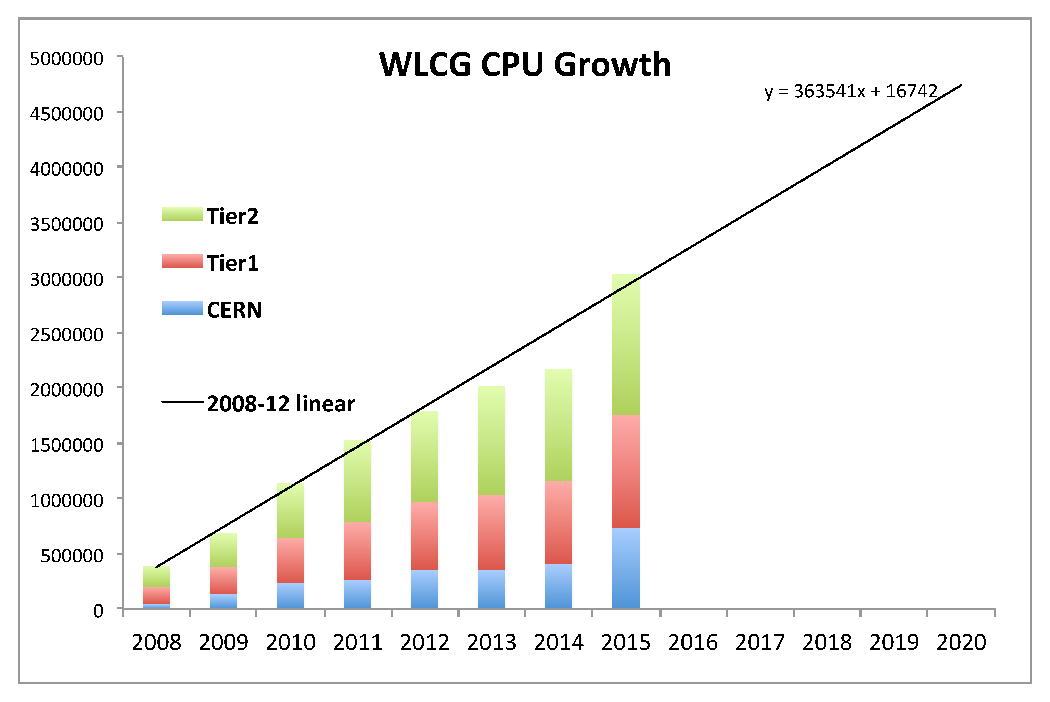
\includegraphics[width=0.45\hsize]{CpF-E2/Growth1.eps}
%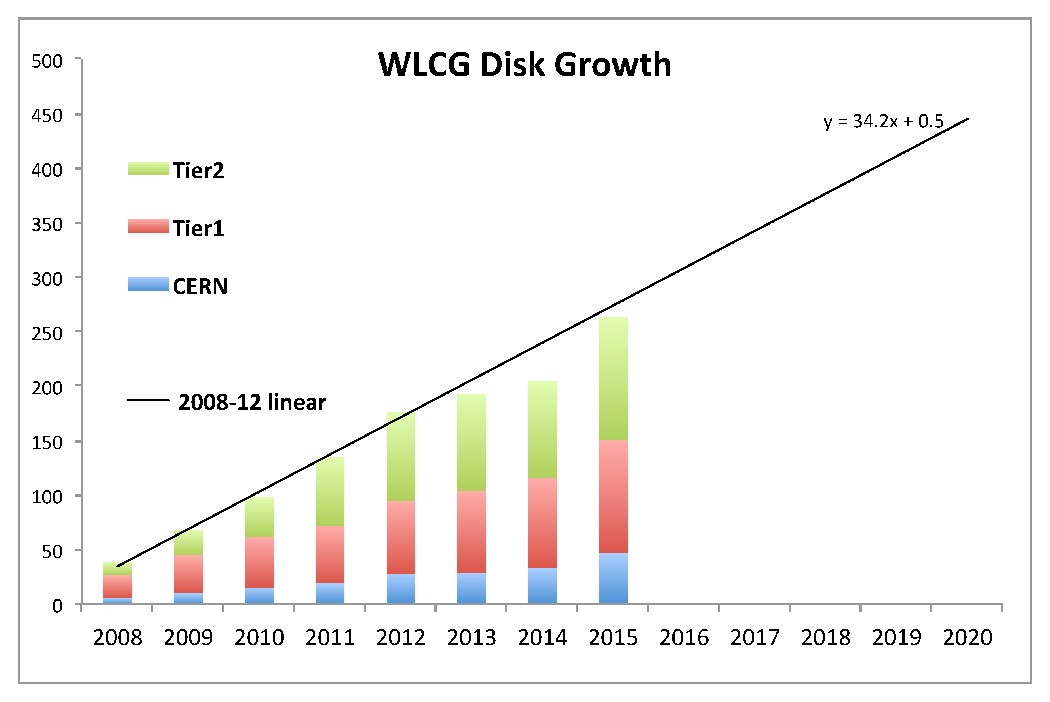
\includegraphics[width=0.45\hsize]{CpF-E2/Growth2.eps}
%\includegraphics{CpF-E2/FigureSnowMass.eps}
\includegraphics[width=0.5\hsize]{CpF-E2/fig1a.pdf}\ \ \ \
\includegraphics[width=0.45\hsize]{CpF-E2/fig1b.pdf}
\caption{The CPU and disk growth through the first 6 years of the LHC program
and projections to 2017.}
\label{fig:growth}
\end{center}
\end{figure}
%%%%%%%%%%%%%%%%%%%%%%%%%%%%%%%%%%%%%%%%%%%%%%%%%%%%%%%%%%%%%%%%%%%%%%%%%%%


Extrapolating the growth trend out 10 years,  LHC computing would have
roughly three times the computing expected in 2015, which is lower than that
predicted by Moore's law.  LHC would reach nearly 800 PB of disk 
space by
2023, which again is roughly a factor of three greater that predicted for
2015.   These increases could
probably be achieved with close to flat budgets.   There are potential
efficiency improvements and new techniques that will be discussed below.

The luminosity and complexity increase dramatically
going to the HL-LHC or other proposed hadron collider programs.
If those plans are realized,  computing would not be on
the curve in Figure~\ref{fig:growth}, but would require a significant shift.
To estimate the increase in resources needed to move from the LHC to the
HL-LHC, it is instructive to examine the transition from the Tevatron to the
LHC.  Data rates are about a factor of ten larger for the LHC at the end
of 2013 than for the Tevatron in 2003.
However,  during that time the total computing
capacity went up by a factor of thirty, while the disk capacity, the local data
served, the wide area networking from the host lab, and the inter-site
transfers all increased by a factor of 100 to accommodate this step.  The step
from LHC Run2 to the HL-LHC will similarly require very significant additional
resources, and quite possibly a disruptive change in technologies and
approaches.
We identify two trends that will potentially help with this: the
increased use of specialized hardware, and providing and using computing as a
service.

\subsection{Trends to specialized systems and computing as a service}
The Energy Frontier will need to evolve to use alternative computing
architectures and platforms such as GPUs and other co-processors,  low-power
``small'' cores, etc., as the focus of industry development is moving away from
the classic server CPU.  Using GPUs introduces significant diversity to the
system, complicates the programming, and changes the approaches used in
scientific calculations, but can increase performance by orders of magnitude
for specific types of calculations.  Co-processors have similar potential
improvement gains, but also increase the diversity and complexity of the
system, and pose additional programming challenges.  Low-power mobile
platforms are most interesting when they are combined into massively parallel,
specialized system in which a single rack 
may have the same number of cores as a
remote computing center does today.  These systems would be used more like a
supercomputer and less like a batch farm, which will require new
expertise in dealing with these more highly interconnected computers.

Specialized hardware and architectures are likely to be deployed initially in
extremely well controlled environments, like trigger farms and other dedicated
centers, where the hardware can be controlled and specified. The next phase is
likely to be schedulable, dedicated, specialized systems that permit large-scale
calculations to achieve a goal similar to making a supercomputer center
request.  Large-scale clusters of specialized hardware owned by the experiment
are likely to come last, and are only likely to come if they can completely
replace a class of computing resources and perform a function at a reduced
cost and higher efficiency.

The other trend impacting Energy Frontier computing is the move to computing as a service
and other ``cloud-based'' solutions.  Currently,  commercial offerings, academic
resources, and opportunistic resources are all being offered through cloud
provisioning techniques.  Opportunistic resources are computers with some amount
of idle unused capacity that can be accessed by communities for free
except for the effort required to make them useful.
While commercial solutions are still more expensive
than well-used dedicated resources, there is a steady decrease in the pricing.

Energy Frontier computing should expect a transition to more shared and opportunistic
resources provided through a variety of interfaces, including cloud
interfaces.   Effort is needed to allow the community to make effective use of
the diverse environments and to perform resource provisioning across
dedicated, specialized, contributed, opportunistic, and purchased resources.

\subsection{Becoming more selective}
There are considerable concerns regarding the enormous increase in data
produced by the next round of Energy Frontier colliders,   to be processed by the offline
computing systems.  We observe that while the Energy Frontier processing capacity has
increased largely as would be expected from Moore's law and relatively
flat budgets, the storage requirements have grown much faster.  The larger
number of sites and the need for local caches, the increase in trigger rates,
and the larger event sizes drive the need for disk-based storage.

For Energy Frontier discovery physics and searches there is a case for storing all
potentially interesting events, and then computationally  applying various
hypotheses to look for new physics.  
Some searches, and many measurements, may benefit from a
new approach where much more of the processing and analysis is done with the
initial data collection and only synthesized output is archived.
This approach has the
potential for preserving physics while reducing the offline processing and
storage needs.  
%%Already the ALICE experiment is planning to do mostly online
%%reconstruction, starting with  the coming running period.   For experiments at
%%future Energy Frontier accelerators there will be strong motivations to reconstruct and
%%calibrate online and write only constants.
%%%{\color{red} Julia has questions about last two sentences}

We expect a change of mentality, moving away from the approach that higher
trigger rates are always better, and that all data from  all triggered events
need to be kept.   As the Energy Frontier trigger rates go up by an order of magnitude,  as
expected for the LHC, and certainly for the HL-LHC,  the experiments
should expect to be more selective in what classes of events will be fully
reconstructed,  and instead develop an approach of on-demand reconstruction,
calibration, and analysis.

Simulation and raw-data reconstruction produce derived data that can
entirely be reproduced. At the LHC, already many of the intermediate steps are
treated as transient data.   More of the data analysis steps should be moved
into the production chain, only storing the final output, with the
understanding that it can be re-derived if required later.

\subsection{Data management}
With the expected increased diversity of computing resources, Energy Frontier computing
needs to develop a data management system that can deal with all kinds of
resources.   In the next decade computing processing for the Energy Frontier will evolve to
be less deterministic, with more emphasis on cloud-provisioned resources,
opportunistic computing, local computing, and volunteer computing.   A data
management system is needed to handle the placement of the data and allow the
operations team and analysis users to concentrate more on execution of work
flows and less on placement and location of data.

Industry has put a focus on delivering content either through Content
Delivery Networks (CDNs) or through peer-to-peer systems.  The experiment data
management systems need to evolve to be more flexible in terms of what 
computing resources can be used to solve each type of computing problem,
in order to make efficient use of the diverse landscape of resoucres to which
the experiment computing modes will have to adapt.
The development of a data intensive content delivery network should not be
unique to one experiment, and should even be applicable to several scientific
domains, but this will require commitment and effort to develop.

Additional details may be found in the full subgroup report 
\cite{Fisk:2014lia}.

